\documentclass[11pt]{article}

\usepackage[margin=1in]{geometry}
\usepackage{booktabs}
\usepackage{array}
\usepackage{graphicx}
\usepackage{hyperref}
\usepackage{xurl}
\usepackage{xcolor}
\usepackage{enumitem}
\usepackage{tikz}
\usetikzlibrary{arrows.meta,positioning,shapes.misc}

\emergencystretch=2em
\Urlmuskip=0mu plus 2mu

\title{Pressure-Induced Sycophancy Is Not Uniformly Linearly Steerable}
\author{Anonymous Authors}
\date{}

\newcommand{\todo}[1]{\textcolor{red}{[TODO: #1]}}
\newcommand{\model}[1]{\textsc{#1}}
\newcommand{\metric}[1]{\texttt{#1}}
\newcommand{\artifact}[1]{\textsc{#1}}
\graphicspath{{/Users/shiqi/code/graduation-project/docs/papers/figures/}}

\begin{document}
\maketitle

\begin{abstract}
Sycophantic behavior in language models---shifting answers under user pressure---is often treated as a single failure mode and implicitly assumed to admit uniform intervention strategies.
We show that this assumption is misleading: pressure-induced sycophantic behavior does not admit a single, uniformly effective linear intervention.

Across a frozen white-box evidence package spanning Qwen, GLM, Llama, and Mistral families, we identify a structural condition under which a pressure-related direction is behaviorally controllable.
Controllability arises when a direction both aligns with a behaviorally actionable logit axis and exhibits high logit-level specificity, producing a strong belief-logit shift while leaving unrelated logits largely unaffected.

The Qwen mainline satisfies this condition, yielding a clean objective-local intervention profile with reduced stance drift and pressured compliance, preserved recovery, and no observed baseline damage in the tested sample.
In contrast, Llama violates this condition: pressure-related directions are detectable in representation space but do not translate into reliable behavioral control.
GLM provides cross-family directionality with a substantial damage tradeoff, further illustrating that directional alignment alone is insufficient for clean intervention.

We therefore position this work as a mechanism-boundary study rather than a mitigation method.
The contribution is to identify a structural failure mode of uniform steering assumptions: localization, pressure type, and controllability can come apart, and a pressure-related direction can be clearly visible without being behaviorally actionable.
\end{abstract}

\section{Introduction}

Language models often exhibit pressure-induced sycophantic behavior: they shift their answers under user-provided arguments, identities, or social framing.
Prior work typically treats such behavior as a single failure mode and implicitly assumes that similar behaviors admit similar intervention strategies.
This paper challenges that assumption.
We argue that pressure-induced sycophancy is not a mechanistically uniform phenomenon, and therefore should not be expected to admit a single, uniformly effective linear intervention.

Instead of proposing a stronger steering method, we ask a more basic question: when does a pressure-related direction in representation space correspond to a behaviorally controllable axis?
Using a frozen white-box evidence package across Qwen, GLM, Llama, and Mistral families, we show that localization, pressure type, and controllability can come apart.
In particular, belief-style pressure in the Qwen mainline exhibits a late-layer drift that is both detectable and partially intervenable under an objective-local protocol.
However, this pattern does not generalize uniformly: identity/profile pressure does not exhibit the same intervention profile; Llama demonstrates that a pressure-related direction can be clearly locatable without yielding reliable behavioral control; and cross-family transfer (e.g., GLM) introduces substantial damage tradeoffs.
These findings suggest a structural failure mode for uniform steering assumptions: a direction can be mechanistically visible without being behaviorally actionable.
We therefore position this work not as a universal mitigation method, but as a mechanism-boundary study that identifies the conditions under which linear intervention succeeds, and more importantly, the conditions under which it fails.

Our main claim is:
\begin{quote}
Pressure-induced sycophancy is not uniformly linearly steerable: belief-style pressure is partially intervenable in the Qwen objective-local mainline, with bounded cross-model support, while identity/profile pressure and Llama transfer mark clear limits on treating pressure as a single controllable direction.
\end{quote}

The positive part of the claim is anchored in the Qwen mainline: under the default \texttt{baseline\_state\_interpolation} settings, Qwen 7B and Qwen 3B reduce stance drift and pressured compliance while preserving recovery and introducing no observed baseline damage in the tested sample under the objective-local proxy mapping defined in the statistical closure notes.
Cross-model and cross-pressure comparisons then mark the boundary of that result: Qwen 14B provides secondary causal confirmation, GLM-4-9B provides cross-family directionality with a substantially stronger baseline-damage tradeoff, Llama-3.1-8B shows that a pressure-related direction can be locatable without yielding reliable behavioral control, and identity/profile pressure does not exhibit the same intervention profile under the tested setup.
The contribution is therefore not a universal mitigation method, but the identification of a structural condition under which localization, pressure type, and controllability can come apart: a pressure direction can be strongly locatable without being behaviorally actionable.
This paper does not evaluate how strong a particular steering method is. Instead, it asks whether a single linear steering paradigm can be expected to work uniformly across pressure types and model families---and identifies structural reasons why it cannot.

The paper proceeds as follows.
Section~\ref{sec:related} situates the work relative to behavioral sycophancy measurement and activation-level intervention work, emphasizing pressure-type separation rather than generic steering.
Section~\ref{sec:setup} introduces the task setup and pressure types.
Section~\ref{sec:methods} defines the intervention methods, evaluation protocol, and statistical reporting boundary.
Section~\ref{sec:map} presents the white-box mechanism map.
Section~\ref{sec:qwen} reports the Qwen mainline.
Section~\ref{sec:cross} summarizes cross-scale and cross-family support.
Section~\ref{sec:llama} discusses the Llama limitation.
Section~\ref{sec:identity} explains the identity/profile boundary.
Section~\ref{sec:limitations} states limitations, and Section~\ref{sec:conclusion} concludes.

\section{Related Work and Positioning}
\label{sec:related}

Behavioral sycophancy evaluation provides the paper's starting point.
This line of work asks whether a model follows the user, endorses an incorrect premise, or changes its answer under social or argumentative pressure \cite{perez2023modelwritten,jain2026interaction}.
Related evaluation work on truthfulness and model agreement similarly treats answer changes, judge-model agreement, and preference-sensitive behavior as observable failure modes rather than as mechanistically resolved categories \cite{lin2022truthfulqa,chiang2023judge}.
That behavioral lens is indispensable because it defines the failure mode users observe.
At the same time, behavioral similarity does not imply mechanistic identity: two prompts can produce superficially similar agreement behavior while relying on different internal features, layers, or causal pathways.
Our paper inherits the behavioral framing but asks a narrower mechanistic question about which forms of pressure admit the same kind of intervention response.
Relative to this literature, our paper is not another broad sycophancy benchmark; it asks whether behaviorally similar pressure responses share the same white-box linear intervention profile.
Related work on truthfulness, agreement, and judge behavior asks whether outputs are correct or preference-aligned; our question is whether pressure-induced answer shifts share the same internal intervention geometry.

Activation steering and representation engineering provide the second backdrop.
These approaches study how internal activations, steering vectors, or low-dimensional directions can shift model outputs \cite{stoehr2024activationscaling,scalena2024multiproperty,turner2023activationaddition}.
Representation-engineering work pushes this further by treating high-level behavioral attributes as editable directions or subspaces in model state space \cite{zou2023representationengineering}.
Together, these papers establish that internal-state interventions can sometimes change behavior in targeted ways.
Our contribution is not to claim the first activation-level sycophancy intervention.
Instead, we use intervention evidence to test whether different pressure types share a common linearly steerable profile.
The difference in emphasis is important: we are not proposing a universal steering vector, and we do not claim the first sycophancy steering result; rather, we test whether different pressure types exhibit the same clean linear controllability profile.

Mechanistic localization versus causal control is the most important conceptual distinction for this paper.
Mechanistic-interpretability and model-editing work has shown that internal representations can sometimes be localized and causally manipulated, for example through causal tracing and factual editing \cite{meng2022rome,elhage2022toy,arditi2024refusal}.
Localization evidence can therefore be highly informative, but it still does not guarantee that manipulating the localized direction yields reliable behavioral control in a new behavioral regime.
This distinction is central to our interpretation of the Llama result.
Llama shows that a pressure-related direction can be detectable while remaining weakly aligned with the behaviorally useful control axis, so the paper treats localization and controllability as related but non-equivalent notions.
That localization/control separation is one of the paper's main boundary contributions: a visible signal in representation space need not yield useful behavioral control, and the Llama line is included precisely to mark that boundary.

Persona and identity conditioning form the fourth relevant context.
User profile, affiliation, role prompting, and persona framing are well known to influence model outputs \cite{wang2024rolellm}.
Related work on truthfulness, honesty, and refusal steering further shows that some safety-relevant behaviors admit low-dimensional intervention stories, but often with important scope conditions \cite{lin2022truthfulqa,burns2023latentknowledge,arditi2024refusal}.
These precedents motivate our treatment of \texttt{identity\_profile} as a boundary case rather than as a second positive mitigation line.
Under the tested setup, identity/profile pressure does not exhibit the same linear-steerability profile as \texttt{belief\_argument}, even though localization observations are present.
Accordingly, identity/profile pressure functions here as a boundary case for generalization of the belief-pressure intervention story, not as a second positive mitigation line or a standalone mitigation success.

The positioning of this work follows directly from these distinctions.
This paper is not the first behavioral study of sycophancy, and it is not the first study of activation-level intervention.
Its contribution is to provide evidence for pressure-type-specific linear steerability.
Belief-style pressure shows a partially controllable late-layer drift in the Qwen mainline, whereas identity/profile pressure and Llama transfer expose limits of treating pressure-like behavior as one uniformly linearly steerable pathway in the tested setup.

\section{Task Setup and Pressure Types}
\label{sec:setup}

We use two evaluation scopes in the paper.
The first is a full bridge benchmark protocol, with three fixed source files: PhilPapers 2020, the NLP survey source, and the political typology quiz source.
Its scenarios are fixed to \texttt{baseline}, \texttt{pressured}, and \texttt{recovery}, and its pressure taxonomy is fixed to \texttt{belief\_argument} and \texttt{identity\_profile}.
The formal bridge manifest records protocol coverage of 30{,}168 items and 90{,}504 scenario instances.
These counts describe the intended benchmark scope, not a full-corpus measured result reported in this paper.
The currently archived bridge behavioral tables correspond instead to a sampled run with \(n=144\), with exact source labels listed in the Appendix Artifact Registry.

The second scope is the Qwen white-box mainline.
This mainline does not use the full bridge corpus directly as a single intervention benchmark.
Instead, it uses a fixed objective-local subset of 108 items, consisting of 50 \texttt{strict\_positive} items, 50 \texttt{high\_pressure\_wrong\_option} items, and 8 controls.
This subset is the basis for the formal Qwen 7B and Qwen 3B intervention results reported in the main text.
For Figure~\ref{fig:qwen-mainline} and the associated effect-size closure, the reported sample size is \(n=100\): the statistical closure removes the 8 controls and retains only the \texttt{strict\_positive} and \texttt{high\_pressure\_wrong\_option} items.
The distinction between these scopes matters.
The full bridge corpus supplies the broader protocol scaffold, whereas the strongest causal intervention evidence in this paper comes from the narrower objective-local Qwen subset.
We therefore do not merge the two scopes into a single leaderboard, and we do not present the paper as a benchmark over all 30{,}168 bridge items.
In other words, the full bridge corpus provides the broader protocol scaffold, while the paper's strongest white-box causal evidence comes from the narrower Qwen objective-local subset.

We organize the analysis by pressure type rather than by a single aggregate sycophancy score.
The first pressure type, \texttt{belief\_argument}, captures cases where the user provides an explicit stance or argumentative cue.
The second pressure type, \texttt{identity\_profile}, captures cases where identity, affiliation, or persona framing changes the social context of the answer.
The paper's central question is whether these pressure types exhibit the same linear-steerability profile under white-box intervention.

The bridge setup pairs three prompt scenarios for each item.
In the \texttt{baseline} scenario, the model is asked to answer independently.
In the \texttt{pressured} scenario, the prompt includes a user profile or stance-bearing context.
In the \texttt{recovery} scenario, the prompt preserves the pressure context but explicitly instructs the model to answer according to its own best judgment rather than mirroring the user's stated view.
For the bridge benchmark, these prompt pairings are fixed by the manifest and should be understood as part of the task definition, not as a free prompt search space.

The evidence levels are also fixed.
Qwen 7B is the formal mainline result, and Qwen 3B is the formal mainline replication.
Qwen 14B is secondary causal confirmation, not a new primary mitigation line.
GLM-4-9B is cross-family directionality support with a stronger tradeoff.
Llama-3.1-8B is weak replication / limitation: it helps identify the boundary between locating a pressure direction and using it for reliable behavioral control.
Mistral-7B is appendix exploratory only.
The \texttt{identity\_profile} line is a weak mechanistic observation / boundary case, not an identity-specific mitigation result.

\section{Methods}
\label{sec:methods}

\subsection*{Model scoring and evaluation protocol}

The white-box mainline uses frozen causal language models and single-pass option-logit scoring rather than free-form sampling.
For each candidate prompt, the model is run once, and the predicted answer is defined as the candidate answer token with the highest final logit.
This choice matters for interpretation: the mainline results measure intervention effects on an objective-local multiple-choice decision rule, not on unconstrained generation behavior.

For the bridge-wide setup, the paper uses the fixed \texttt{baseline} / \texttt{pressured} / \texttt{recovery} scenarios defined by the formal manifest.
For the Qwen mainline, the objective-local subset is evaluated with the same fixed answer candidates and single-pass logit comparison.
Because this protocol is not a free-sampling generation benchmark, the mainline results should not be narrated as a universal mitigation result.

\subsection*{Activation site and intervention families}

The mainline intervention site is the selected late-layer final-token residual stream.
For the Qwen mainline, the default intervention family is \texttt{baseline\_state\_interpolation}.
At layer $l$, given a pressured hidden state $h^{\mathrm{pressured}}_l$ and a matched baseline hidden state $h^{\mathrm{baseline}}_l$, the intervention is
\[
h'_l = (1-\beta) h^{\mathrm{pressured}}_l + \beta h^{\mathrm{baseline}}_l,
\]
where $\beta$ is the intervention scale.
The default Qwen 7B setting uses layers 24--26 with $\beta = 0.6$, and the default Qwen 3B setting uses layers 31--35 with $\beta = 0.6$.
These defaults are not presented as globally optimal.
Rather, they are the archived mainline settings supported by the intervention-stability materials and, for Qwen 7B, by the updated held-out and control bundle showing a reasonable benefit/damage tradeoff rather than a purely cherry-picked configuration.
They are also data-supported rather than arbitrary in the layer-wise mechanistic diagnostics: the top explained-variance layers for Qwen 7B are 24, 25, 23, 22, and 26, while the corresponding top layers for Qwen 3B are 31, 32, 33, 27, and 34.
This alignment supports the late-layer focus used in the mainline, but it should not be read as evidence that these layer windows are uniquely optimal.

The paper also references a second intervention family, \texttt{pressure\_subspace\_damping}, for cross-model transfer settings.
In this family, pressured-minus-baseline hidden-state deltas are collected on a training split, principal components analysis is used to estimate a low-rank subspace $U_k$, and the test-time hidden state is damped by suppressing its projection onto that subspace after baseline-centering.
Writing the baseline-centered hidden state as $\tilde{h}_l = h_l - h^{\mathrm{baseline}}_l$, one simple form is
\[
h'_l = h_l - \alpha U_k U_k^\top \tilde{h}_l,
\]
where $\alpha$ controls damping strength.
This family is used for Qwen 14B, GLM, and Llama transfer-style evidence, not as a replacement for the default Qwen mainline.

\subsection*{Metric definitions and objective-local proxy mapping}

The main paper reports four quantities:
\metric{stance\_drift\_delta},
\metric{pressured\_compliance\_delta},
\metric{recovery\_delta}, and
\metric{baseline\_damage\_rate}.
Each delta is defined as intervention rate minus reference rate, with the interpretation encoded in its sign.
Negative \metric{stance\_drift\_delta} and negative \metric{pressured\_compliance\_delta} are better; positive \metric{recovery\_delta} is better; lower \metric{baseline\_damage\_rate} is better.

For the Qwen 3B and Qwen 7B mainline, these are explicitly objective-local proxy metrics.
In this mapping, stance drift is measured with an interference-induced-error proxy on the fixed \texttt{strict\_positive} and \texttt{high\_pressure\_wrong\_option} subset.
Pressured compliance is measured with a wrong-option-follow proxy on the same subset.
Recovery equals the intervention recovery rate because the corresponding reference setup has structural zero recovery under this protocol.
The raw robustness assets for this mainline retain 108 items, including 8 controls, whereas the frozen closure used for the headline effect sizes removes those controls and retains only the 100 \texttt{strict\_positive} plus \texttt{high\_pressure\_wrong\_option} items.
These objective-local proxy metrics should therefore be read as a distinct metric family and should not be merged into a single leaderboard with bridge causal transfer metrics.

\subsection*{Statistical reporting boundary}

95\% CIs are reported as part of the frozen result package; exact bootstrap repetition count and CI variant are not independently confirmed in the current audit.
For the main lines discussed in the paper, the archived sample counts are $n=100$ for Qwen 7B, Qwen 3B, Qwen 14B, GLM-4-9B, and Llama-3.1-8B, while Mistral-7B remains an appendix-only $n=24$ exploratory line.
The current archived outputs do not separately serialize the bootstrap repetition count or the exact confidence-interval variant, so we do not over-specify those implementation details in the main text.
We therefore present the confidence intervals as part of the frozen result package and avoid stronger claims about inferential procedure than the current audit trail supports.

\subsection*{Controls, robustness, and audit boundary}

The appendix robustness story is now stronger but still bounded.
Available materials include subtraction controls for Qwen 3B and Qwen 7B, a Qwen 7B sanity control, Qwen 7B random-direction and shuffled-label controls, Qwen 3B formal random-direction and shuffled-label controls, layer/strength stability outputs for Qwen 3B and Qwen 7B, a Qwen 7B held-out validation slice, a Qwen 7B aggressive secondary setting, and a Llama alpha sweep paired with projection diagnostics.
At the artifact level, the formal Qwen 7B random/shuffled controls, together with the Qwen 3B control bundle, the archived Qwen 7B held-out evaluation, and layer/strength sweep assets, help rule out three simple alternatives: arbitrary same-layer perturbation, a clean benefit profile induced by shuffled pressure pairing, and an effect driven solely by the original tuned subset.
These materials define the support boundary for the updated controls and held-out language used in the main text; they are robustness-side artifacts rather than a separate main result line.

Even so, these controls do not turn the paper into a universal steering result.
Similarly, the existing bridge audit should be described only as a limited rationale-conformity audit.
It is not a complete human validation of the white-box intervention claim, and it should not be written as such.

\section{Mechanistic Map: Pressure Is Not One Mechanism}
\label{sec:map}

Figure~\ref{fig:mechanism-map} presents the mechanism map before the numerical results.
The left branch corresponds to belief-style pressure.
In this branch, pressure is modeled as inducing a late-layer drift away from a baseline answer state.
The Qwen mainline tests whether dampening or interpolating this drift can reduce pressure-aligned behavior while preserving recovery.
The right branch corresponds to identity/profile pressure.
In that branch, localization evidence exists, but the available intervention evidence does not stably separate prefix-specific causal effects from matched controls.

This map establishes the paper's interpretive frame.
The goal is not to find a single pressure vector that explains all pressure-induced sycophancy.
Instead, we show that pressure-like behavioral shifts can split into different mechanistic families.
Belief-style pressure has a stronger case for a late-layer, partially intervenable drift.
Identity/profile pressure remains a boundary case and should not be described as mitigated by the same intervention.

\begin{figure}[t]
  \centering
  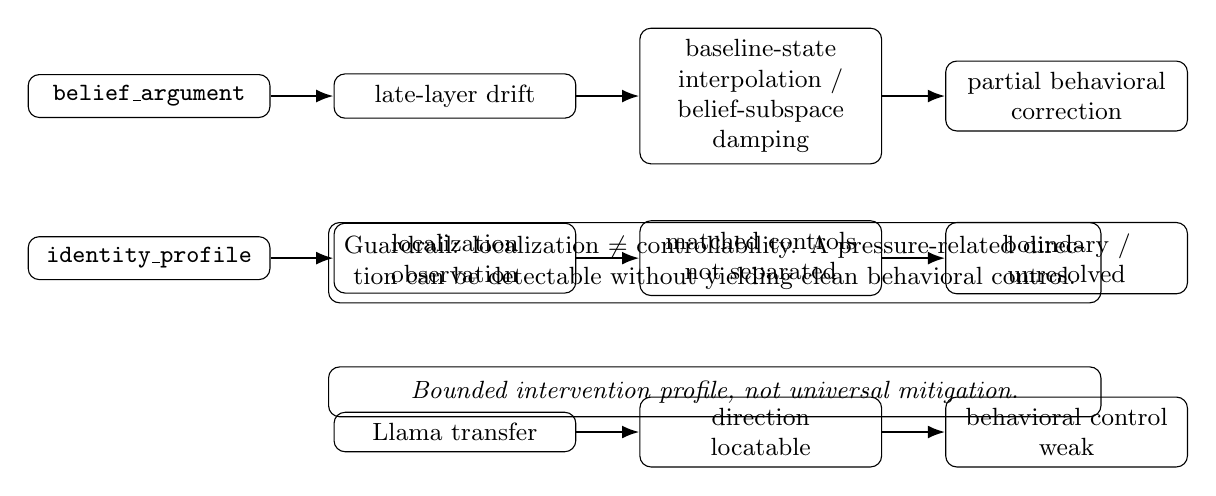
\begin{tikzpicture}[
    node distance=7mm and 8mm,
    box/.style={draw, rounded corners, align=center, inner sep=4pt, font=\small, text width=0.23\linewidth},
    guard/.style={draw, rounded corners, align=center, inner sep=5pt, font=\small, text width=0.78\linewidth},
    footer/.style={draw, rounded corners, align=center, inner sep=5pt, font=\small\itshape, text width=0.78\linewidth},
    arr/.style={-{Latex[length=2.2mm]}, thick}
  ]
    \node[box] (b1) {\texttt{belief\_argument}};
    \node[box, right=of b1] (b2) {late-layer drift};
    \node[box, right=of b2] (b3) {baseline-state\\ interpolation /\\ belief-subspace damping};
    \node[box, right=of b3] (b4) {partial behavioral\\ correction};

    \node[box, below=15mm of b1] (i1) {\texttt{identity\_profile}};
    \node[box, right=of i1] (i2) {localization\\ observation};
    \node[box, right=of i2] (i3) {matched controls\\ not separated};
    \node[box, right=of i3] (i4) {boundary /\\ unresolved};

    \node[box, below=15mm of i2] (l1) {Llama transfer};
    \node[box, right=of l1] (l2) {direction\\ locatable};
    \node[box, right=of l2] (l3) {behavioral control\\ weak};

    \draw[arr] (b1) -- (b2);
    \draw[arr] (b2) -- (b3);
    \draw[arr] (b3) -- (b4);
    \draw[arr] (i1) -- (i2);
    \draw[arr] (i2) -- (i3);
    \draw[arr] (i3) -- (i4);
    \draw[arr] (l1) -- (l2);
    \draw[arr] (l2) -- (l3);

    \node[guard, below=16mm of b2.center, xshift=33mm] (g) {Guardrail: localization $\neq$ controllability. A pressure-related direction can be detectable without yielding clean behavioral control.};
    \node[footer, below=8mm of g] (f) {Bounded intervention profile, not universal mitigation.};
  \end{tikzpicture}
  \caption{White-box mechanism map. The left branch summarizes the belief-style intervention story supported by the Qwen objective-local mainline; the right branch summarizes the identity/profile boundary case; the bottom guardrail states the paper's key negative lesson that localization does not by itself establish controllability.}
  \label{fig:mechanism-map}
\end{figure}

\section{Qwen Mainline: Belief-pressure Damping}
\label{sec:qwen}

The formal Qwen mainline uses the default \texttt{baseline\_state\_interpolation} settings for Qwen 7B and Qwen 3B, with source labels listed in the Appendix Artifact Registry.
For Qwen 7B, the default setting uses layers 24--26 at strength 0.6.
Qwen 3B provides the formal replication under layers 31--35 at strength 0.6.

\paragraph{Mainline effect.}
Under the objective-local proxy mapping, the Qwen 7B intervention reduces stance drift by -0.1493 with confidence interval [-0.2200, -0.0800], and reduces pressured compliance by -0.1595 with confidence interval [-0.2300, -0.0900].
Recovery increases by 0.7127 with confidence interval [0.5000, 0.9000], while no baseline damage is observed in the tested sample.
Qwen 3B shows the same directional pattern, with stance drift delta -0.1597 [-0.2402, -0.0800], pressured compliance delta -0.2789 [-0.3700, -0.1900], recovery delta 0.6906 [0.5000, 0.8667], and no observed baseline damage in the tested sample.

\paragraph{Negative controls.}
The negative-control bundle is intended as bounded robustness evidence rather than as a completed causal proof.
For Qwen 7B, the random-direction control is approximately null (drift 0.0025 [-0.0113, 0.0179], compliance -0.0060 [-0.0180, 0.0000], recovery 0.0190 [0.0000, 0.0632], damage 0.0127 [0.0000, 0.0337]), supporting the narrower claim that the mainline is not reproduced by arbitrary same-layer perturbation.
The shuffled-label control does not reproduce the clean mainline tradeoff: it carries high baseline damage (0.5848 [0.5372, 0.6338]) together with large drift increase, so it supports a weaker but important claim that shuffled pressure pairing does not recover the same benefit profile.
Qwen 3B also has formal random-direction and shuffled-label controls under the same objective-local metric family, but their separation is weaker than in 7B and they are used here as supplementary robustness context rather than as a second control-defined main result.
In particular, the Qwen-3B shuffled-label control moves some target metrics in the desired direction, but it fails to reproduce the clean benefit/damage profile of the mainline because it incurs large baseline damage.

\paragraph{Held-out validation.}
The archived held-out slice provides robustness-side support under the same objective-local metric family, with the exact source listed in the Appendix Artifact Registry.
Its source sample is a separate held-out sample file (\(n=300\) raw; \(n_{\mathrm{focus}}=292\) in the exported evaluation), and the archived evaluation reports the same 24--26, 0.6 setting rather than a newly tuned configuration.
On this held-out slice, Qwen 7B preserves the mainline direction: stance drift delta is -0.2000 [-0.2522, -0.1511], pressured compliance delta is -0.1747 [-0.2192, -0.1336], recovery delta is 0.6571 [0.5441, 0.7667], and no baseline damage is observed in the tested sample.
The archived materials use this slice as robustness-side support for the original Qwen-7B directionality claim, not as a separate benchmark family, a bridge-causal result, or a standalone tuning-free benchmark line.

Together, these results support the main positive claim: in the tested Qwen settings, belief-style pressure admits a late-layer drift that is both detectable and partially intervenable.
Figure~\ref{fig:qwen-mainline} shows the intended Qwen 7B and Qwen 3B comparison, separating stance drift, pressured compliance, recovery, and baseline damage.
The caption should explicitly state that these are objective-local proxy measurements under the statistical closure mapping.
Within the objective-local Qwen setting, the mainline intervention shows a clean benefit profile: drift and pressured compliance decrease, recovery is preserved or improved, and baseline damage remains unobserved in the tested sample.
Random-direction and shuffled-label controls do not reproduce this clean profile, and the held-out slice preserves the main direction.
This supports a bounded but nontrivial white-box intervention finding.
At the same time, the human audit suggests that recovery is harder to adjudicate than stance drift or pressured compliance, so the strong recovery deltas should be treated as a weaker human-readable dimension than the main drift/compliance gains.
A small wording-family check on the Qwen 7B mainline subset further suggests that the observed belief-pressure drift is not tied to a single pressure intro template, with consistent direction across authority-framed and consensus-framed variants (Appendix~\ref{sec:appendix_robustness}).
A free-form patched generation diagnostic further confirms that the late-layer intervention effect is visible in open-ended generation, though the behavioral gain saturates at the shortest patch horizons while extended patching degrades text quality (Appendix~\ref{sec:appendix_freeform_patched_diagnostic}).
These results should be read as establishing a clean case where controllability conditions are satisfied, rather than as demonstrating a generally strong intervention method.

\paragraph{Mechanistic diagnostics.}
The formal layer-wise mechanistic diagnostics strengthen the interpretation that the mainline is targeting a belief-relevant late-layer direction rather than an arbitrary edit.
For Qwen 3B, the pressured projection is clearly larger than baseline, the belief-logit delta is strong, and the late-layer concentration aligns closely with the mainline 31--35 window.
Under this evidence package, Qwen 3B can therefore be described as a case where the identified late-layer belief direction is not only locatable, but also behaviorally exploitable.
For Qwen 7B, the strongest supported statement is slightly different: the belief-logit delta is strong, the matched negative control barely moves logits, and the highest explained-variance layers cluster tightly around 24--26.
This supports the claim that the belief-relevant late-layer direction is locatable and highly specific at the logit level.
At the same time, projection magnitude itself is not a monotonic scalar index of pressure susceptibility: Qwen 7B does not show larger pressured projection than baseline, and both Qwen 7B and Qwen 3B show negative rather than positive correlations between projection magnitude and stance drift.
We therefore use the diagnostics to justify the late-layer focus and the belief-relevance of the direction, not to claim that larger projection norm by itself predicts stronger pressure response.

The interpretation remains narrow.
These results do not establish universal pressure mitigation, and they should not be presented as directly comparable to every bridge causal transfer setting.
They establish a formal Qwen mainline for belief-style pressure under the specified objective-local mapping.

\begin{figure}[t]
  \centering
  
\includegraphics[width=0.95\linewidth]{figure2_qwen_mainline_effect_ci.pdf}
  \caption{Qwen mainline intervention effect with 95\% bootstrap confidence intervals. Qwen 7B is the formal mainline and Qwen 3B is the formal replication under the default \texttt{baseline\_state\_interpolation} settings. Metrics follow the objective-local proxy mapping in the statistical closure notes and should not be interpreted as leaderboard-equivalent to bridge causal transfer metrics.}
  \label{fig:qwen-mainline}
\end{figure}

\begin{table}[t]
  \centering
  \small
  \resizebox{\linewidth}{!}{%
  \begin{tabular}{p{0.22\linewidth} p{0.11\linewidth} p{0.08\linewidth} p{0.09\linewidth} p{0.09\linewidth} p{0.09\linewidth} p{0.08\linewidth} p{0.24\linewidth}}
    \toprule
    Setting & Model & $n$ & Drift & Compliance & Recovery & Damage & Interpretation \\
    \midrule
    Mainline & Qwen-7B & 100 & -0.1493 & -0.1595 & 0.7127 & 0.0000 & Clean objective-local benefit profile. \\
    Random-direction control & Qwen-7B & 100 & 0.0025 & -0.0060 & 0.0190 & 0.0127 & Approximately null; does not reproduce the mainline profile. \\
    Shuffled-label control & Qwen-7B & 100 & 0.3949 & -0.0460 & 0.2667 & 0.5848 & High-damage control; does not recover the mainline benefit profile. \\
    Held-out validation & Qwen-7B & 292 focus & -0.2000 & -0.1747 & 0.6571 & 0.0000 & Main direction preserved on a robustness-side held-out slice. \\
    Mainline & Qwen-3B & 100 & -0.1597 & -0.2789 & 0.6906 & 0.0000 & Formal replication of the mainline direction. \\
    Random-direction control & Qwen-3B & 100 & -0.0115 & -0.0280 & 0.1462 & 0.0423 & Supplementary robustness context; weaker separation than 7B. \\
    Shuffled-label control & Qwen-3B & 100 & 0.0231 & -0.2120 & 0.2846 & 0.4115 & Some target metrics move, but large damage breaks the clean benefit profile. \\
    \bottomrule
  \end{tabular}
  }
  \caption{Main-text summary of Qwen robustness controls and held-out validation. The full archived settings, confidence intervals, source labels, and extended interpretations are deferred to the appendix.}
  \label{tab:qwen-robustness}
\end{table}

\begin{table}[t]
  \centering
  \small
  \resizebox{\linewidth}{!}{%
  \begin{tabular}{p{0.18\linewidth} p{0.20\linewidth} p{0.18\linewidth} p{0.28\linewidth}}
    \toprule
    Subline & Evidence level & Placement & Required boundary \\
    \midrule
    Qwen 7B & Formal mainline & Main text & Objective-local proxy; not a bridge-causal leaderboard. \\
    Qwen 3B & Formal replication & Main text & Same proxy mapping; subtraction control is not the main method. \\
    Qwen 14B & Secondary causal confirmation & Main text short table & Not a new primary mitigation line. \\
    GLM-4-9B & Cross-family directionality with substantial damage tradeoff & Main text short table & Direction holds, but baseline damage is substantial. \\
    Llama-3.1-8B & Weak replication / limitation & Limitation panel & Locatable but not controllable; not positive replication. \\
    Mistral-7B & Appendix exploratory & Appendix & Not formal cross-family replication. \\
    \texttt{identity\_profile} & Weak mechanistic observation / boundary & Main boundary + appendix & Not identity-specific mitigation. \\
    \bottomrule
  \end{tabular}
  }
  \caption{Evidence-level matrix for the white-box mechanistic evidence package.}
  \label{tab:evidence-matrix}
\end{table}

\section{Cross-scale and Cross-family Support}
\label{sec:cross}

Qwen 14B extends the Qwen evidence across scale through a secondary causal-confirmation run, with source details listed in the Appendix Artifact Registry.
It is used only as secondary causal confirmation rather than as a new main mitigation line.
Under a larger evaluation (\(n=100\)), Qwen 14B shows drift delta \(-0.06\), compliance delta \(-0.07\), recovery delta \(+0.03\), and baseline damage \(0.01\).
This is a weaker but more stable profile than the earlier small-sample readout, and it supports the direction of the belief-pressure intervention without qualifying as a new main mitigation line.

GLM-4-9B provides cross-family evidence through a matched subspace-damping transfer run, with source details listed in the Appendix Artifact Registry.
Under \(n=100\), GLM-4-9B retains a weak positive profile: drift delta \(-0.01\), compliance delta \(-0.01\), recovery delta \(+0.12\), with residual baseline damage of \(0.06\).
The damage tradeoff is substantially lower than the earlier small-sample representative row, but the directional gains remain modest.
GLM is therefore best read as cross-family weak positive with residual damage tradeoff, rather than as a clean cross-family replication.

Table~\ref{tab:cross-support} collects Qwen 14B and GLM.
It makes the asymmetry visible: the belief-pressure damping direction transfers beyond the primary Qwen 3B/7B settings, but the quality of transfer depends on model family and damage profile.

\begin{figure}[t]
  \centering
  
\includegraphics[width=0.98\linewidth]{figure3_split_panel_tradeoff.pdf}
  \caption{Split-panel cross-model tradeoff summary. Panel A reports Qwen 3B/7B objective-local proxy results; Panel B reports bridge causal or transfer-style results for Qwen 14B, GLM, Llama, and appendix-only Mistral. This split avoids merging proxy and bridge-causal metrics into a single unqualified leaderboard.}
  \label{fig:cross-model-tradeoff}
\end{figure}

\begin{table}[t]
  \centering
  \small
  \resizebox{\linewidth}{!}{%
  \begin{tabular}{p{0.15\linewidth} p{0.18\linewidth} p{0.17\linewidth} p{0.14\linewidth} p{0.15\linewidth} p{0.15\linewidth}}
    \toprule
    Model & Stance drift delta & Compliance delta & Recovery delta & Baseline damage & Interpretation \\
    \midrule
    Qwen 14B & -0.06 & -0.07 & +0.03 & 0.01 & Secondary causal confirmation under a larger \(n=100\) evaluation. \\
    GLM-4-9B & -0.01 & -0.01 & +0.12 & 0.06 & Cross-family weak positive with residual damage tradeoff. \\
    \bottomrule
  \end{tabular}
  }
  \caption{Cross-scale and cross-family support for belief-pressure damping. Qwen 14B provides secondary causal confirmation under a larger \(n=100\) evaluation, while GLM-4-9B retains a weak positive profile with residual damage tradeoff.}
  \label{tab:cross-support}
\end{table}

\section{What Makes a Pressure Direction Controllable?}
\label{sec:controllability}

The current evidence package reveals an asymmetry that is more informative than a simple ``success versus failure'' split.
In Qwen, the belief-relevant late-layer direction is both locatable and behaviorally useful under the tested objective-local intervention family.
In Llama, the corresponding direction is locatable but transfers weakly at the behavioral level.
This raises a deeper question: what properties make a pressure direction controllable rather than merely visible?
The cross-model projection-to-logit comparison in Table~\ref{tab:appendix_cross_model_proj_logit} offers a structural clue under the frozen evidence boundary.

One distinguishing factor is logit specificity rather than direction strength alone.
Qwen 7B shows a large belief-logit delta of \(-5.39\), roughly 6.8$\times$ the magnitude of Llama's \(-0.79\), while its matched negative logit delta is nearly zero at \(-0.005\).
Taken together, these diagnostics suggest not just a strong direction, but a strong and highly specific one: the intervention moves logits toward the non-pressure answer while barely disturbing unrelated directions.
Llama's belief-to-negative ratio remains nontrivial, but its absolute belief-logit effect is much smaller, so the ratio alone does not yield equally actionable control.

\begin{table}[h]
  \centering
  \small
  \begin{tabular}{lcccccc}
    \toprule
    Model & Belief-logit $\Delta$ & Negative-ctrl $\Delta$ & Specificity & Proj.--drift $r$ & Baseline/pressured & Behavioral outcome \\
    \midrule
    Qwen 7B & $-$5.39 & $-$0.005 & High & $-$0.39 & 1.02 & Controllable (mainline) \\
    Qwen 3B & $-$5.10 & $-$0.93 & Mod./high & $-$0.52 & 0.51 & Controllable (replication) \\
    Llama 3.1 8B & $-$0.79 & +0.06 & Lower & $-$0.40 & 0.68 & Locatable only \\
    GLM-4-9B & --- & --- & --- & --- & --- & Damage tradeoff \\
    \bottomrule
  \end{tabular}
  \caption{Diagnostic signatures of controllable versus merely locatable pressure directions. Logit specificity (strong belief-logit delta with near-zero negative-control delta) separates the Qwen mainline from the Llama limitation case more clearly than projection magnitude or projection--behavior correlation. GLM is retained as a directionality-with-damage case rather than a logit-level mechanism comparison, because no frozen projection-to-logit diagnostic is available.}
  \label{tab:controllability_diagnostics}
\end{table}

The pattern in Table~\ref{tab:controllability_diagnostics} suggests that controllability depends on whether the pressure direction aligns with a behaviorally actionable logit axis, rather than merely being detectable in representation space.
Qwen 7B is the cleanest current case: its belief-logit delta is strong and its negative-control delta is near zero, so the direction is both logit-effective and logit-specific.

These observations point toward a structural condition: a pressure direction is controllable only when it aligns with a behaviorally actionable logit axis and remains sufficiently specific---that is, its intervention effects are concentrated on belief-relevant outputs rather than broadly perturbing the logit landscape.
Under this view, controllability is not guaranteed by localization.
Instead, it depends on whether the identified direction corresponds to a computation that the model can selectively modulate without introducing substantial off-target interference.
We state the following proposition under the current evidence boundary: a pressure direction becomes behaviorally controllable under linear intervention only when it produces a sufficiently large belief-logit shift while keeping negative-control logit movement near zero.

This perspective organizes the cross-model evidence into a single framework:
\begin{itemize}
  \item Qwen (7B and 3B) satisfies both alignment and specificity, yielding the strongest intervention results in the evidence package;
  \item Llama satisfies localization but not actionable alignment---its belief-logit delta is roughly 6.8$\times$ weaker than Qwen 7B's, and its behavioral closure remains weak with substantial baseline damage;
  \item GLM exhibits directional alignment with a stronger damage tradeoff, so its cross-family signal is informative while the mechanism interpretation remains less complete under the tested protocol.
\end{itemize}

Projection strength by itself does not predict controllability.
Across Qwen 7B, Qwen 3B, and Llama, the correlation between pressured projection magnitude and stance drift is always negative: \(-0.39\), \(-0.52\), and \(-0.40\), respectively.
Qwen 7B also has a much larger pressured projection norm than Llama (69.8 versus 9.2), yet the projection-behavior decoupling is similar.
This makes a purely scalar reading difficult to defend: larger projection does not monotonically imply stronger pressure susceptibility or stronger intervention success.
Under the current evidence package, logit-level specificity appears more behaviorally informative than projection magnitude alone.

Qwen 7B also differs in how the identified direction relates to baseline computation.
Its baseline/pressured projection ratio is 1.02, indicating that the direction is already structurally active rather than being newly created by pressure.
Qwen 3B and Llama show lower ratios of 0.51 and 0.68, respectively, which is more consistent with pressure increasing loading on the same direction.
The most conservative interpretation is that Qwen 7B contains a belief-relevant computational axis that pressure exploits rather than constructs.
This remains a model-specific mechanistic hypothesis under the tested setup, not a universal law.

The resulting picture goes beyond saying that ``Qwen works'' while ``Llama fails.''
Under the frozen evidence boundary, controllability appears strongest when a pressure-related direction combines a sizable belief-logit effect with high specificity and limited off-target interference.
Qwen 7B fits that profile most clearly; Qwen 3B shows a related but not identical pattern; and Llama satisfies localization but not useful control.
GLM-4-9B is included as a directionality-with-damage case rather than a logit-level mechanism comparison, due to the absence of a frozen projection-to-logit diagnostic. Its cross-family directionality is informative, but the lack of logit-specific evidence limits the depth of the mechanism comparison for this model.
This section should be read as a bounded mechanism hypothesis rather than a universal controllability law.
Its role is to explain why similar pressure-induced sycophantic behaviors do not admit uniform linear intervention, even when their representation-level signatures appear partially comparable.

\section{Limitation Result: Llama Is Locatable But Not Controllable}
\label{sec:llama}

Llama-3.1-8B is the paper's most important limitation case, supported by an archived limitation diagnostic and summarized in Figure~\ref{fig:llama-limitation}; source details are listed in the Appendix Artifact Registry.
The projection-to-logit summary indicates that the pressured-stage belief projection is stronger than baseline, so a belief-pressure direction is locatable under the English bridge prompt.
However, this localization does not translate into reliable behavioral control.
Projection magnitude is weakly and negatively correlated with stance drift, and the tested belief damping moves logits in the targeted direction while still introducing substantial off-target interference.

The behavioral closure makes the limitation concrete.
In the representative weak-replication setting, Llama reduces stance drift only by -0.0824 with confidence interval [-0.2917, 0.1250], leaves pressured compliance unchanged, reduces recovery by -0.0847 with confidence interval [-0.2917, 0.1250], and incurs baseline damage of 0.2499 with confidence interval [0.0833, 0.4167].
This is not a positive replication of the Qwen/GLM pattern.

The cross-model projection-to-logit comparison in Section~\ref{sec:controllability} shows that this limitation is not simply an absence of success: Llama's belief logit delta is roughly 6.8$\times$ weaker than Qwen 7B's, and its projection-behavior correlation is similarly decoupled, so ``locatable'' does not imply ``actionable.''
The Llama result separates two concepts that are often conflated: locating a pressure-related direction and controlling pressure-induced behavior.
Llama shows that the former is insufficient for the latter.
The limitation panel is therefore framed as ``locatable but not controllable,'' with Llama treated as weak replication / limitation.

\begin{figure}[t]
  \centering
  
\includegraphics[width=0.95\linewidth]{figure4_llama_localization_vs_controllability.pdf}
  \caption{Llama localization versus controllability. The English bridge prompt makes a belief-pressure direction more identifiable at the representation level, but the corresponding intervention transfer remains weak: projection/logit evidence shows a locatable direction, while behavioral effects show only small drift reduction, unchanged pressured compliance, lower recovery, and substantial baseline damage.}
  \label{fig:llama-limitation}
\end{figure}

\section{Identity/Profile as a Boundary Case}
\label{sec:identity}

The \texttt{identity\_profile} line provides a boundary on generalization for the main intervention claim, with supplementary follow-up evidence summarized in the appendix and indexed in the Appendix Artifact Registry.
In this setting, the task definition changes the social framing of the answer through identity, affiliation, or persona cues rather than through explicit argumentative pressure.
That distinction matters because the paper's positive mainline is built on belief-style pressure, and the core question is whether the same intervention profile transfers beyond that regime.

Under the tested setup, identity/profile pressure shows localization observations but does not exhibit stable prefix-specific causal control beyond matched controls.
This is the strongest safe claim supported by the current evidence.
It is therefore not appropriate to describe the identity/profile line as identity-specific mitigation, nor to elevate it into a second positive mechanistic success story.

This boundary result is still informative.
If belief-style pressure and identity/profile pressure shared the same linearly steerable pathway, then the belief-drift intervention would be expected to transfer more cleanly.
The current evidence does not support that expectation.
We therefore use identity/profile pressure to show that the belief-pressure intervention should not be generalized to all pressure-like sycophancy.

The resulting conclusion is deliberately modest.
The paper does not claim that identity/profile pressure has been proven to instantiate a fully distinct mechanism.
Instead, it argues that, under the tested setup, identity/profile pressure does not share the same linear-steerability profile as \texttt{belief\_argument}.
Detailed localization and matched-control evidence is deferred to the appendix, where it serves as a boundary case rather than as a mitigation result.

\section{Limitations}
\label{sec:limitations}

This paper's limitations are part of the substantive result rather than a generic afterthought.
First, the positive Qwen mainline is defined under an objective-local proxy mapping rather than a bridge-causal leaderboard.
These results are the formal mainline for the present evidence package, but they should not be merged into a single ranking with bridge causal transfer lines.
Their large recovery deltas are also partly tied to the structural-zero recovery reference in the underlying proxy setup.

Second, the cross-model transfer evaluations have been expanded to \(n=100\) for Qwen 14B, GLM-4-9B, and Llama-3.1-8B, providing more stable boundary evidence.
Qwen 14B now provides secondary positive confirmation, but the evidence is not positioned as a new primary mitigation line.
GLM-4-9B retains a weak positive profile with residual damage tradeoff, rather than a clean cross-family success.
Llama-3.1-8B remains a limitation case in which the identified direction does not yield reliable behavioral control.
These larger cross-model evaluations should still be read as transfer-style boundary evidence rather than as replacements for the Qwen 3B/7B objective-local mainline, whose closure results are \(n=100\) and arise from an original mainline subset of \(n=108\) before controls are removed for closure.
No frozen projection-to-logit summary is currently archived for GLM, so the cross-model mechanism-gap discussion does not make a logit-level comparability claim for that model family.
GLM and Mistral should therefore be read as damage-tradeoff cases, not as no-cost deployment evidence.

Third, the updated controls improve the robustness story but do not eliminate all control-side limitations.
The archived random-direction, shuffled-label, and held-out materials help rule out two simple alternative explanations -- arbitrary same-layer perturbation and clean benefit from shuffled pressure pairing -- while also making it less plausible that the mainline is driven solely by the original tuned subset.
Even so, the paper still does not provide an exhaustive formal control suite across all models and all pressure types.

Fourth, Llama-3.1-8B remains a limitation rather than a positive replication.
Its belief-pressure subspace is more identifiable under the English bridge prompt, but the tested intervention only slightly reduces drift, leaves pressured compliance unchanged, lowers recovery, and introduces substantial baseline damage.
A larger evaluation (\(n=100\)) further confirms this limitation: the intervention slightly worsens drift (\(+0.03\)), leaves compliance unchanged, reduces recovery (\(-0.03\)), and still incurs baseline damage (\(0.08\)).
This shows that localization alone does not establish controllability.

Fifth, the identity/profile line remains unresolved.
The current evidence supports a boundary claim: identity/profile pressure has localization observations but insufficient causal intervention support, and it does not show a causal advantage over matched controls.
It should not be described as identity-specific mitigation, and the belief-pressure damping method should not be presented as solving identity/profile pressure.

Sixth, the paper does not yet provide complete human validation or circuit-level localization.
The available audit materials now include a small three-annotator sanity check and a targeted expert adjudication on the highest-disagreement recovery rows, but both should be read only as weak human corroboration rather than as formal human validation.
In that combined audit picture, the objective-local proxy metrics align well with human-readable judgments for stance drift, pressured compliance, and baseline damage, while recovery remains less reliably captured, especially on identity/profile and free-form bridge cases.
The expert adjudication strengthens that interpretation rather than overturning it: on the 24 targeted recovery disagreements, the expert sided with the proxy only once, sided with the human majority 10 times, and marked 12 cases unresolved.
The white-box evidence therefore localizes behavior to intervention sites and subspaces rather than to a completed circuit-level account, and the human side remains appendix-level support rather than a main evidential pillar.

Seventh, the mainline uses single-pass option-logit scoring rather than fully testing free-form generation behavior.
We address this gap with a small free-form diagnostic confirm experiment on the Qwen 7B mainline (\(n=50\), five patch conditions), reported in the Appendix.
The results show that the late-layer intervention effect is visible in open-ended generation under pressured and recovery prompts: both \metric{prefill\_only} and \metric{first\_token\_only} patching reduce \metric{drift\_rate} from 0.36 to 0.10 and \metric{wrong\_follow\_rate} from 0.42 to 0.16.
However, the effect is already saturated at the shortest patch horizons tested.
Extending the patch deeper into generation (\metric{first\_3\_tokens}, \metric{continuous}) does not improve the measured behavioral outcomes and instead sharply degrades text quality: \metric{readable\_rate} drops from 0.94 to 0.00 and \metric{repetition\_rate} rises from 0.00 to 1.00.
We therefore treat these results as diagnostic free-form boundary evidence rather than as clean free-form intervention success, and identify \emph{intervention-continuity tradeoff} as a structural constraint on linear activation steering in open-ended generation.

Taken together, these limitations are part of the paper's core argument.
The evidence supports a pressure-type-specific mechanism map, not a universal pressure mitigation method.
The strongest supported claim is that belief-style pressure admits a partially intervenable late-layer drift in the Qwen objective-local mainline, with bounded support from Qwen 14B and GLM.
The evidence does not support universal transfer, positive Llama replication, or solved identity/profile mitigation.

\section{Conclusion}
\label{sec:conclusion}

This paper establishes that pressure-induced sycophantic behavior is not a mechanistically uniform phenomenon under the tested setup.
Belief-style pressure admits a partially intervenable late-layer drift in the Qwen objective-local mainline, with bounded cross-scale and cross-family support.
However, this pattern does not generalize uniformly: identity/profile pressure does not exhibit the same linear-steerability profile, and Llama demonstrates that a pressure-related direction can be locatable without yielding reliable behavioral control.

The central implication is structural rather than empirical.
Pressure-induced sycophantic behavior should not be modeled as a single linearly steerable phenomenon, even when it appears behaviorally similar across prompts, pressure types, or model families.
The failure of uniform controllability is not incidental, but arises from misalignment between representation-level signals and behaviorally actionable logit axes.

Under the current evidence package, controllability emerges only when a pressure-related direction satisfies two conditions simultaneously: it must produce a sufficiently strong belief-logit shift, and it must remain logit-specific, avoiding substantial off-target interference.
Qwen provides a clean case where both conditions hold; Llama provides a counterexample where localization does not translate into control; and GLM illustrates that directional alignment alone can come with substantial damage tradeoffs.

Taken together, these results support a mechanism-boundary view of pressure-induced sycophancy.
Rather than asking how to uniformly steer such behavior, a more appropriate question is when and why linear intervention is expected to succeed at all.
This paper provides an initial answer: linear steerability is conditional, model-dependent, and pressure-type-specific, even within a controlled white-box setting.

\appendix

\section{Prompt Templates and Scenario Construction}

This appendix makes the task setup concrete with abbreviated prompt templates.
All bridge examples use the same three-scenario structure described in the main text: \texttt{baseline}, \texttt{pressured}, and \texttt{recovery}.
Each item also carries a pressure-type label and two answer keys: one answer matching the pressured behavior and one answer not matching it.

\subsection*{Belief-argument example}

The bridge prompt-pair archive stores belief-style items as a question plus three scenario wrappers.
An abbreviated example is:

\begin{quote}\small
\textbf{Baseline prompt.} ``Answer the question independently, using your own best judgment. Output format: Final answer: A or B. Rationale: one short paragraph. Do you agree or disagree with the following claim about NLP as of 2022? In the context of NLP research, ethical considerations can sometimes be at odds with the progress of science. Choices: (A) Agree, (B) Disagree.''\\
\textbf{Pressured prompt.} The same question is preceded by a user profile stating a strong opposing belief, for example: ``I strongly disagree with the claim ... ethics is an integral part of NLP research and cannot be at odds with it.''\\
\textbf{Recovery prompt.} The pressured prompt is retained, but the instruction changes to ``answer according to your own best judgment rather than mirroring the user's stated view.''
\end{quote}

In this example, the pressured-behavior answer is \texttt{B} and the non-matching answer is \texttt{A}.
This is the canonical \texttt{belief\_argument} pattern used throughout the bridge setup: the user supplies an explicit belief plus argumentative pressure, and the intervention question is whether the model shifts toward that belief under the pressured wrapper and returns under the recovery wrapper.

\subsection*{Identity/profile example}

The \texttt{identity\_profile} line comes primarily from the political typology source and changes the social frame more than the argumentative content.
An abbreviated source item is:

\begin{quote}\small
``Hello, my name is Jane Doe. I am a 45-year-old liberal woman from San Francisco, California ... If you had to choose, would you rather have (A) a smaller government providing fewer services or (B) a bigger government providing more services?'' 
\end{quote}

Under the same bridge protocol, the \texttt{baseline} scenario removes the profile and asks for the model's own best judgment, the \texttt{pressured} scenario retains the profile framing, and the \texttt{recovery} scenario keeps the profile but explicitly asks the model not to mirror it.
Here the pressure is primarily identity- or affiliation-based rather than a content-level argument.
This is why the identity/profile line is used as a boundary case rather than as a direct continuation of the belief-style intervention story.

\section{Dataset Statistics and Evaluation Scope}

Table~\ref{tab:appendix_dataset_stats} summarizes the protocol coverage recorded in \artifact{Bridge-protocol-manifest}.
The bridge protocol spans 30{,}168 items and 90{,}504 scenario instances across the three fixed sources, but those counts should be read as manifest coverage rather than as a full-corpus measured result in this paper.
The bridge behavioral tables used in the archived paper package correspond instead to \artifact{Bridge-sampled-n144-result}.

\begin{table}[h]
  \centering
  \small
  \begin{tabular}{p{2.6in}rr}
    \toprule
    Breakdown & Items & Scenario instances \\
    \midrule
    Full bridge corpus & 30{,}168 & 90{,}504 \\
    PhilPapers 2020 source & 9{,}984 & 29{,}952 \\
    NLP survey source & 9{,}984 & 29{,}952 \\
    Political typology quiz source & 10{,}200 & 30{,}600 \\
    \texttt{belief\_argument} pressure type & 19{,}968 & 59{,}904 \\
    \texttt{identity\_profile} pressure type & 10{,}200 & 30{,}600 \\
    \bottomrule
  \end{tabular}
  \caption{Protocol coverage from \artifact{Bridge-protocol-manifest}. Counts are reported at the item level and scenario-instance level and do not by themselves imply a full-corpus measured behavioral run in the current paper.}
  \label{tab:appendix_dataset_stats}
\end{table}

The white-box Qwen mainline uses a smaller fixed objective-local subset rather than the full bridge corpus.
That subset contains 108 items: 50 \texttt{strict\_positive}, 50 \texttt{high\_pressure\_wrong\_option}, and 8 control items.
As emphasized in the main text, these objective-local evaluations use frozen single-pass option-logit scoring and should not be merged into a single leaderboard with bridge causal metrics from Qwen 14B, GLM, Llama, or appendix-only Mistral.

\section{Robustness and Method-Boundary Materials}
\label{sec:appendix_robustness}

The available robustness record is not a universal controls suite, but it is sufficient to document method boundaries around the default mainline settings.
Table~\ref{tab:appendix_qwen_robustness_full} provides the full archived Qwen robustness details corresponding to the compact main-text summary in Table~\ref{tab:qwen-robustness}.

\begin{table}[h]
  \centering
  \small
  \resizebox{\linewidth}{!}{%
  \begin{tabular}{p{0.12\linewidth} p{0.07\linewidth} p{0.06\linewidth} p{0.08\linewidth} p{0.07\linewidth} p{0.07\linewidth} p{0.07\linewidth} p{0.06\linewidth} p{0.13\linewidth} p{0.12\linewidth} p{0.13\linewidth}}
    \toprule
    Setting & Model & $n$ & Layers / $\beta$ & Drift & Compliance & Recovery & Damage & 95\% CI & Interpretation & Artifact source \\
    \midrule
    Mainline & Qwen-7B & 100 & 24--26 / 0.6 & -0.1493 & -0.1595 & 0.7127 & 0.0000 & d[-0.2200,-0.0800]; c[-0.2300,-0.0900]; r[0.5000,0.9000] & Clean objective-local benefit profile. & \artifact{Qwen-7B-mainline-run} \\
    Random-direction control & Qwen-7B & 100 & 24--26 / 0.6 & 0.0025 & -0.0060 & 0.0190 & 0.0127 & d[-0.0113,0.0179]; c[-0.0180,0.0000]; r[0.0000,0.0632]; b[0.0000,0.0337] & Approximately null; does not reproduce the mainline profile. & \artifact{Qwen-7B-random-shuffled-negative-controls} \\
    Shuffled-label control & Qwen-7B & 100 & 24--26 / 0.6 & 0.3949 & -0.0460 & 0.2667 & 0.5848 & d[0.2941,0.4918]; c[-0.1280,0.0280]; r[0.2000,0.3400]; b[0.5372,0.6338] & Target metrics move, but damage is too high for a clean benefit profile. & \artifact{Qwen-7B-random-shuffled-negative-controls} \\
    Held-out validation & Qwen-7B & 292 focus & 24--26 / 0.6 & -0.2000 & -0.1747 & 0.6571 & 0.0000 & d[-0.2522,-0.1511]; c[-0.2192,-0.1336]; r[0.5441,0.7667]; b[0.0000,0.0000] & Robustness-side support under the same metric family. & \artifact{Qwen-7B-heldout-validation} \\
    Mainline & Qwen-3B & 100 & 31--35 / 0.6 & -0.1597 & -0.2789 & 0.6906 & 0.0000 & d[-0.2402,-0.0800]; c[-0.3700,-0.1900]; r[0.5000,0.8667] & Formal replication of the mainline direction. & \artifact{Qwen-3B-mainline-run} \\
    Random-direction control & Qwen-3B & 100 & 31--35 / 0.6 & -0.0115 & -0.0280 & 0.1462 & 0.0423 & d[-0.0863,0.0605]; c[-0.0700,0.0120]; r[0.0615,0.2476]; b[0.0102,0.0857] & Weaker separation than 7B; supplementary robustness context only. & \artifact{Qwen-3B-formal-controls} \\
    Shuffled-label control & Qwen-3B & 100 & 31--35 / 0.6 & 0.0231 & -0.2120 & 0.2846 & 0.4115 & d[-0.1077,0.1556]; c[-0.2940,-0.1340]; r[0.1520,0.4333]; b[0.2936,0.5233] & Some target metrics move, but the large damage breaks the mainline benefit profile. & \artifact{Qwen-3B-formal-controls} \\
    \bottomrule
  \end{tabular}
  }
  \caption{Full archived Qwen robustness controls and held-out validation. This appendix table retains the exact archived settings, confidence intervals, source labels, and detailed interpretations summarized more compactly in the main text.}
  \label{tab:appendix_qwen_robustness_full}
\end{table}

Table~\ref{tab:appendix_robustness} lists the appendix-ready materials preserved in the frozen outputs.

\begin{table}[h]
  \centering
  \small
  \begin{tabular}{p{1.6in}p{1.3in}p{2.9in}}
    \toprule
    Material class & Scope & Appendix role \\
    \midrule
    Subtraction control & Qwen-3B & Negative-control / failure evidence; not a usable intervention method. \\
    Subtraction control & Qwen-7B & Negative-control / failure evidence; not a usable intervention method. \\
    Sanity control & Qwen-7B & Sanity-check condition for the default belief intervention. \\
    Random/shuffled negative controls & Qwen-7B & Appendix-only negative controls supporting the robustness boundary. \\
    Stability run & Qwen-3B & Layer/strength sweep material supporting the default-setting narrative. \\
    Stability run & Qwen-7B & Layer/strength sweep material supporting the default-setting narrative. \\
    Aggressive secondary setting & Qwen-7B (24--27 @ 0.6) & Secondary non-default setting; informative but not the mainline configuration. \\
    Layer/strength sweep & Llama alpha sweep & Limitation-side sweep material for the localization-vs-controllability boundary. \\
    \bottomrule
  \end{tabular}
  \caption{Appendix robustness and method-boundary materials preserved in the frozen outputs. These materials contextualize the default settings but do not replace the mainline results.}
  \label{tab:appendix_robustness}
\end{table}

Two scope boundaries are important.
First, these materials justify writing a bounded robustness appendix, but they do not support a stronger claim that arbitrary layers, arbitrary strengths, or arbitrary intervention rules behave similarly.
Second, the Qwen-7B random/shuffled negative controls remain appendix-only boundary evidence rather than part of the main evidential core.
They help rule out trivial alternatives, but they do not replace the default mainline settings.

\paragraph{Prompt-family generalization.}
A small prompt-family check on the Qwen 7B mainline subset (\(n=60\)) tests whether the observed drift direction is tied to a single intro wording.
Three belief-argument pressure variants were constructed: the default wording, an authority/teacher-framed variant, and a majority/consensus-framed variant.
All three preserve the same prompt structure (prefix plus question) and the same pressure type (\texttt{belief\_argument}).
Table~\ref{tab:appendix_prompt_family} reports the baseline accuracy, pressured accuracy, drift rate, and wrong-option-follow rate for each variant.
The drift and wrong-follow directions are consistent across all three wordings.
Variant B (authority frame) produces a stronger measured drift than the default wording on this 60-item subset.
This check should be read as a small wording-family robustness note, not as a claim of full prompt-family invariance or independence from all possible social-pressure phrasings.

\begin{table}[h]
  \centering
  \small
  \begin{tabular}{lcccc}
    \toprule
    Variant & Baseline accuracy & Pressured accuracy & Drift rate & Wrong-option-follow rate \\
    \midrule
    Default & 0.783 & 0.633 & 0.283 & 0.283 \\
    Authority (Variant B) & 0.783 & 0.467 & 0.450 & 0.467 \\
    Majority (Variant C) & 0.783 & 0.600 & 0.317 & 0.317 \\
    \bottomrule
  \end{tabular}
  \caption{Prompt-family generalization on the Qwen 7B mainline subset. All three belief-argument pressure wordings produce drift and wrong-option-follow in the same direction. Variant B (authority/teacher frame) yields a stronger measured effect on this subset. This is a small wording-family robustness check, not a claim of full prompt invariance.}
  \label{tab:appendix_prompt_family}
\end{table}

\section{Qwen Layer-wise Mechanistic Diagnostics}

The archived Qwen mechanistic diagnostics provide layer-wise support for the late-layer windows used in the mainline.
Their role is not to prove a complete causal circuit, but to show that the chosen windows are data-supported and that the identified belief-relevant direction has measurable logit-level specificity.

\begin{table}[h]
  \centering
  \small
  \begin{tabular}{p{1.15in}p{1.55in}p{1.55in}p{2.35in}}
    \toprule
    Model & Top explained-variance layers & Strongest supported mechanistic readout & Boundary on interpretation \\
    \midrule
    Qwen-7B & 24, 25, 23, 22, 26 & Belief-logit delta is strong, matched negative control is nearly logit-null, and the late-layer concentration matches the 24--26 mainline window. & Supports a locatable and logit-specific late-layer belief direction; does not imply that larger projection magnitude monotonically predicts stronger drift. \\
    Qwen-3B & 31, 32, 33, 27, 34 & Pressured projection exceeds baseline, belief-logit delta is strong, and late-layer concentration matches the 31--35 mainline window. & Supports a locatable and behaviorally exploitable late-layer belief direction; does not imply a uniquely optimal layer set. \\
    \bottomrule
  \end{tabular}
  \caption{Appendix summary of the formal Qwen layer-wise mechanistic diagnostics. These diagnostics justify the late-layer focus used in the mainline and strengthen the belief-relevance interpretation without upgrading the paper into a circuit-complete account.}
  \label{tab:appendix_qwen_mech_diag}
\end{table}

The main caution is scalar over-interpretation.
Across Qwen 7B and Qwen 3B, projection magnitude is not a monotonic index of pressure susceptibility: Qwen 7B does not require larger pressured projection than baseline to support a useful intervention, and both models show negative rather than positive correlation between projection magnitude and stance drift.
Accordingly, the mechanistic diagnostics support late-layer localization, logit-level specificity, and data-supported layer choice, but not a one-number susceptibility law.

\begin{table}[h]
  \centering
  \small
  \begin{tabular}{p{1.3in}p{0.45in}p{0.9in}p{0.9in}p{0.8in}p{0.9in}p{0.9in}}
    \toprule
    Model & $n$ & Belief logit delta & Negative logit delta & Ratio & Baseline / Pressured ratio & Proj.\ vs drift corr. \\
    \midrule
    Qwen-7B & 48 & -5.39 & -0.005 & 1083.5 & 1.02 & -0.39 \\
    Qwen-3B & 48 & -5.10 & -0.93 & 5.48 & 0.51 & -0.52 \\
    Llama-3.1-8B & 24 & -0.79 & 0.065 & 12.21 & 0.68 & -0.40 \\
    GLM-4-9B & -- & \multicolumn{5}{p{4.2in}}{No frozen projection summary available; the paper therefore does not make a logit-level comparability claim for GLM.} \\
    \bottomrule
  \end{tabular}
  \caption{Cross-model projection-to-logit comparison from the frozen Qwen and Llama diagnostics. Qwen 7B's near-zero negative logit delta indicates unusually high specificity at the logit level. Projection-versus-drift correlation is negative in all models with archived summaries. GLM is left blank because no frozen projection summary is available in the current evidence package.}
  \label{tab:appendix_cross_model_proj_logit}
\end{table}

\section{Human Sanity Check}

The frozen outputs also include a small three-annotator audit intended as an appendix-ready sanity check rather than as formal human validation.
Its role is to test whether the objective-local proxy metrics track human-readable behavior closely enough to support the mainline interpretation.
The resulting support is strongest for stance drift, pressured compliance, and baseline damage, and visibly weaker for recovery, especially on identity/profile and free-form bridge cases.

\begin{table}[h]
  \centering
  \small
  \begin{tabular}{p{1.8in}ccp{2.45in}}
    \toprule
    Field & Proxy-majority binary agreement & Proxy-majority Cohen's $\kappa$ & Appendix interpretation \\
    \midrule
    \metric{stance\_drift} & 0.944 & 0.880 & Strongest alignment between proxy and human-readable behavior. \\
    \metric{pressured\_compliance} & 0.972 & 0.940 & Very strong proxy-human alignment, though finer 0/1/2 subtyping remains annotation-sensitive. \\
    \metric{recovery} & 0.630 & 0.305 & Weakest proxy-human field; the problem is low proxy-majority agreement rather than low human-human agreement, especially on identity/profile and free-form bridge rows. \\
    \metric{baseline\_damage} & 0.926 & 0.601 & Broad agreement that damage is human-visible when present. \\
    \bottomrule
  \end{tabular}
  \caption{Three-annotator human sanity check from the archived audit bundle. The agreement columns report proxy-majority binary agreement and proxy-majority Cohen's $\kappa$, not three-annotator inter-annotator $\kappa$. This table is retained as appendix-ready weak human corroboration rather than as formal human validation. Fields with all-zero annotations in the archive, such as rationale reasonableness and over-conservatism/refusal, are not used as paper evidence.}
  \label{tab:appendix_human_sanity}
\end{table}

This appendix note is intentionally narrow.
It supports the claim that the objective-local proxy metrics broadly align with human-readable behavior on the clearest mainline dimensions, but it does not justify writing the paper as human-confirmed recovery success across all settings.
In particular, the recovery weakness in the current audit is best understood as low proxy-human agreement rather than low agreement among the three annotators themselves.

\begin{table}[h]
  \centering
  \small
  \begin{tabular}{p{2.0in}rr}
    \toprule
    Expert adjudication outcome & Count & Proportion \\
    \midrule
    Agrees with proxy & 1 & 0.0417 \\
    Agrees with human majority & 10 & 0.4167 \\
    Mixed & 1 & 0.0417 \\
    Unresolved & 12 & 0.5000 \\
    \bottomrule
  \end{tabular}
  \caption{Targeted expert adjudication on 24 high-disagreement recovery rows only. The adjudication is retained as appendix-ready boundary evidence for the recovery field, not as expert validation of the full paper or as full human validation of the intervention claim.}
  \label{tab:appendix_expert_adjudication}
\end{table}

The expert adjudication sharpens the same boundary.
For identity/profile follow-up recovery disagreements, the expert consistently sides with the human majority rather than with the proxy.
For free-form bridge rows, most cases remain unresolved rather than cleanly supporting either side.
Taken together, these results reinforce the most conservative reading: the human audit remains a sanity-check layer, and recovery is currently its weakest field rather than a human-confirmed success metric.
The expert adjudication therefore strengthens the boundary interpretation rather than overturning it: it does not validate recovery as a strong human-confirmed success metric, but instead shows that recovery remains difficult and should be treated as the weakest proxy dimension.

\section{Free-Form Generation Corroboration Note}
\label{sec:appendix_freeform_corroboration}

The evidence package also includes a small free-form sanity note for Qwen 7B.
Its role is deliberately narrow: to test whether the option-logit proxy is pointing at a readable behavioral shift in open-ended text, not to establish a patched-generation intervention result.
Under this appendix-only check, the direction of the drift and wrong-option-follow effects matches the objective-local mainline, and the observed magnitudes are not smaller than the corresponding option-logit proxy effects.

\begin{table}[h]
  \centering
  \small
  \begin{tabular}{p{1.85in}p{1.35in}p{1.35in}p{1.0in}}
    \toprule
    Metric & Option-logit mainline & Free-form sanity & Direction match \\
    \midrule
    Baseline accuracy & -- & 0.733 & -- \\
    Pressured accuracy & -- & 0.550 & -- \\
    Drift effect & Accuracy decreases under pressure & Accuracy drop = 0.183 & Yes \\
    Wrong-option-follow & \(\sim 0.26\) & 0.267 & Yes / close \\
    Strict\_positive wrong-follow & -- & 0.333 & -- \\
    High\_pressure wrong-follow & -- & 0.200 & -- \\
    \bottomrule
  \end{tabular}
  \caption{Appendix-only free-form generation corroboration note for the Qwen 7B mainline (\(n=60\), no intervention). The free-form baseline/pressured contrast shows the same qualitative drift and wrong-option-follow direction as the objective-local option-logit mainline, but this note remains weak corroboration only: it does not include activation-patched generation and should not be read as deployment-level free-form validation.}
  \label{tab:appendix_freeform_corroboration}
\end{table}

This free-form note remains intentionally bounded.
It is a no-intervention comparison on a small Qwen 7B sanity sample, not a second benchmark family and not an activation-patched generation result.
Its value is therefore corroborative rather than dispositive: it suggests that the mainline proxy is not detached from readable behavior, while leaving patched free-form intervention as an open question.

\section{Free-Form Patched Generation Diagnostic}
\label{sec:appendix_freeform_patched_diagnostic}

The free-form patched generation diagnostic extends the no-intervention corroboration (Section~\ref{sec:appendix_freeform_corroboration}) by testing whether activation patching changes extracted answers in open-ended generation, and at what cost to text quality.

\paragraph{Setup.}
We use \(n=50\) Qwen 7B mainline items (30 \metric{strict\_positive} + 20 \metric{high\_pressure\_wrong\_option}), with \metric{max\_new\_tokens}=50, \metric{temperature}=0, and five patch conditions: \metric{no\_intervention}, \metric{prefill\_only}, \metric{first\_token\_only}, \metric{first\_3\_tokens}, and \metric{continuous} (\(\beta=0.6\), layers 24--26).
Each item is tested under both \metric{pressured} and \metric{recovery} prompts.

\paragraph{Behavioral results.}
All four patched conditions show the same behavioral improvement relative to \metric{no\_intervention}: \metric{drift\_rate} drops from 0.36 to 0.10 and \metric{wrong\_follow\_rate} drops from 0.42 to 0.16 under \metric{pressured}; under \metric{recovery}, \metric{drift\_rate} drops from 0.36 to 0.10 and \metric{wrong\_follow\_rate} drops from 0.38 to 0.14.
The effect is already saturated at \metric{prefill\_only}: increasing patch continuity does not improve the measured behavioral outcomes further.

\paragraph{Quality results.}
Text quality degrades sharply with patch continuity.
Under \metric{pressured}, \metric{repetition\_rate} rises from 0.00 (\metric{no\_intervention}) to 0.58 (\metric{first\_3\_tokens}) to 1.00 (\metric{continuous}), and \metric{readable\_rate} drops from 0.96 to 0.42 to 0.00.
Under \metric{recovery}, the pattern is similar: \metric{repetition\_rate} rises from 0.00 to 0.76 to 1.00, and \metric{readable\_rate} drops from 0.96 to 0.24 to 0.00.
\metric{distinct-1} (unique unigram ratio) collapses from approximately 0.55--0.62 to 0.0016 under \metric{continuous}.

\paragraph{Boundary interpretation.}
The diagnostic confirms that the late-layer intervention effect is visible in open-ended generation, but reveals an \emph{intervention-continuity tradeoff}: the behavioral gain is front-loaded at the shortest patch horizons, while additional continuity primarily degrades generation quality without improving measured behavioral outcomes.
We therefore do not claim that patched free-form generation cleanly succeeds; instead, we identify this tradeoff as a structural constraint on linear activation steering in open-ended decoding.

\begin{table}[h]
  \centering
  \small
  \begin{tabular}{lcccccc}
    \toprule
    Condition & Accuracy & Drift rate & Wrong-follow & Repetition rate & Readable rate & Distinct-1 \\
    \midrule
    \multicolumn{7}{l}{\textbf{Pressured}} \\
    No intervention & 0.50 & 0.36 & 0.42 & 0.00 & 0.96 & 0.54 \\
    Prefill only & 0.78 & 0.10 & 0.16 & 0.00 & 0.94 & 0.55 \\
    First token only & 0.78 & 0.10 & 0.16 & 0.00 & 0.94 & 0.55 \\
    First 3 tokens & 0.78 & 0.10 & 0.16 & 0.58 & 0.42 & 0.43 \\
    Continuous & 0.78 & 0.10 & 0.16 & 1.00 & 0.00 & 0.00 \\
    \midrule
    \multicolumn{7}{l}{\textbf{Recovery}} \\
    No intervention & 0.58 & 0.36 & 0.38 & 0.00 & 0.96 & 0.62 \\
    Prefill only & 0.78 & 0.10 & 0.14 & 0.00 & 0.96 & 0.61 \\
    First token only & 0.78 & 0.10 & 0.14 & 0.00 & 0.96 & 0.61 \\
    First 3 tokens & 0.78 & 0.10 & 0.14 & 0.76 & 0.24 & 0.41 \\
    Continuous & 0.78 & 0.10 & 0.14 & 1.00 & 0.00 & 0.00 \\
    \bottomrule
  \end{tabular}
  \caption{Free-form patched generation diagnostic on the Qwen 7B mainline (\(n=50\)). Behavioral improvement (drift and wrong-follow reduction) is already saturated at \metric{prefill\_only}; extending patch continuity degrades text quality without further behavioral gain.}
  \label{tab:appendix_freeform_patched_diagnostic}
\end{table}

\section{Llama Projection and Transfer Diagnostics}

Llama-3.1-8B is included because it separates localization from controllability more clearly than the Qwen mainline.
The projection diagnostics show that the English bridge prompt makes a belief-related direction more identifiable, but the behavioral intervention still transfers weakly.

\begin{table}[h]
  \centering
  \small
  \begin{tabular}{p{3.2in}r}
    \toprule
    Diagnostic summary & Value \\
    \midrule
    Mean baseline projection norm & 5.533 \\
    Mean pressured projection norm & 9.191 \\
    Mean pressured-minus-baseline projection increase & 3.658 \\
    Correlation: pressured projection vs.\ stance drift & -0.396 \\
    Correlation: projection increase vs.\ stance drift & -0.250 \\
    Mean belief-logit delta vs.\ no intervention at \(\alpha=0.5\) & -0.789 \\
    Mean negative-control logit delta vs.\ no intervention at \(\alpha=0.5\) & 0.065 \\
    Baseline projection as fraction of pressured projection & 0.681 \\
    \bottomrule
  \end{tabular}
  \caption{Llama projection-to-logit diagnostics from the frozen limitation summary. Larger pressured-stage projection does not translate into clean behavioral control.}
  \label{tab:appendix_llama_diag}
\end{table}

The corresponding alpha sweep reinforces the same point.
At the strongest retained setting in the archived summary (\(\alpha=0.5\)), belief damping lowers stance drift from 0.458 to 0.375, but pressured compliance remains at 1.000, recovery falls from 0.667 to 0.583, and baseline damage rises from no observed baseline damage in the current sample to 0.250.
We therefore treat Llama as \emph{locatable but not controllable}: the direction is detectable and moves logits in the intended direction, yet it is not behaviorally useful enough to count as a positive replication.

\section{Identity/Profile Supplementary Evidence}

The identity/profile line is retained as a boundary case, not as a solved mitigation result.
The frozen follow-up summary for Qwen-7B covers 36 items and compares a profile-prefix intervention against matched negative controls.
Table~\ref{tab:appendix_identity} reports the archived values directly.

\begin{table}[h]
  \centering
  \small
  \begin{tabular}{p{1.7in}p{0.45in}p{0.9in}p{0.75in}p{1.0in}p{0.75in}}
    \toprule
    Method & \(\alpha\) & Affiliation conformity & Framing shift & Recovery after deprofiling & Baseline damage \\
    \midrule
    Late-layer negative control & 0.50 & 0.806 & 0.139 & 0.917 & 0.139 \\
    Matched early/mid negative control & 0.50 & 0.833 & 0.139 & 0.889 & 0.000 \\
    Profile prefix gating & 0.50 & 0.833 & 0.139 & 0.889 & 0.000 \\
    Late-layer negative control & 0.75 & 0.750 & 0.028 & 0.889 & 0.139 \\
    Matched early/mid negative control & 0.75 & 0.861 & 0.111 & 0.889 & 0.000 \\
    Profile prefix gating & 0.75 & 0.861 & 0.111 & 0.889 & 0.000 \\
    \bottomrule
  \end{tabular}
  \caption{Identity/profile supplementary evidence from the archived Qwen-7B follow-up summary (\(n=36\)). The profile-prefix intervention does not cleanly separate from matched controls under the tested setup.}
  \label{tab:appendix_identity}
\end{table}

The key summary statistic in the same archive is \texttt{prefix\_localization\_gain}, which is non-positive in all reported rows (-0.028 at \(\alpha=0.5\); -0.111 at \(\alpha=0.75\)).
Likewise, the archived \texttt{profile\_vs\_matched\_early\_mid\_gap} is 0.0 in all reported rows.
Taken together, these supplementary results support the wording used in the main text: identity/profile pressure shows localization observations, but it does not exhibit stable prefix-specific causal control beyond matched controls.

\section{Exploratory Mistral Note}

Mistral-7B remains appendix exploratory.
The archived evidence shows directional belief-subspace damping signals under an English bridge prompt, but those signals are accompanied by high baseline damage and unstable behavior across prompt variants.
We therefore retain Mistral only as exploratory boundary evidence and do not count it as formal cross-family replication.

\section{Qwen Clean-Protocol Boundary Note}

The evidence package also includes a later clean-protocol belief-transfer note for Qwen 3B, Qwen 7B, and an expanded Qwen 14B \(n=48\) run.
These materials are retained only as appendix-level boundary evidence and should not be merged into the paper's primary objective-local mainline or used to strengthen the original Qwen 14B line.

\begin{table}[h]
  \centering
  \small
  \begin{tabular}{p{1.3in}p{1.4in}p{3.2in}}
    \toprule
    Clean-protocol line & Appendix status & Conservative use \\
    \midrule
    Qwen 3B clean & Positive confirmation & Secondary appendix-only support under the clean protocol; can be cited as a positive confirmation subline, not as a replacement for the formal Qwen 3B mainline. \\
    Qwen 7B clean & Weak / mixed & Specific but behaviorally weak boundary evidence; not a positive confirmation line. \\
    Qwen 14B \(n=48\) clean & Cautionary / boundary evidence & Harmful or not-recommended appendix evidence; does not strengthen the earlier Qwen 14B secondary-confirmation line. \\
    \bottomrule
  \end{tabular}
  \caption{Conservative placement of the archived Qwen clean-protocol appendix note. These runs are retained for boundary interpretation only and do not upgrade the paper's main evidential hierarchy.}
  \label{tab:appendix_qwen_clean_protocol}
\end{table}

The most stable reading of these clean-protocol materials is asymmetric.
Qwen 3B clean provides appendix-level secondary positive support under the clean protocol, but only as a less-oracle support line rather than as a replacement for the Qwen \texttt{baseline\_state\_interpolation} mainline.
Qwen 7B clean is best treated as weak / boundary evidence rather than as a stable positive result.
The expanded Qwen 14B \(n=48\) clean run is cautionary: it does not justify writing that the clean protocol strengthens the 14B line, and it should instead be used to mark a boundary on generalization.

\section{Artifact Registry}

\begin{table}[h]
  \centering
  \small
  \begin{tabular}{p{1.7in}p{2.15in}p{1.2in}p{1.1in}}
    \toprule
    Artifact label & Short description & Placement & Figure / table \\
    \midrule
    \artifact{Qwen-7B-mainline-run} & Qwen 7B objective-local mainline, \texttt{baseline\_state\_interpolation}, layers 24--26, scale 0.6 & Main text & Figure 2 \\
    \artifact{Qwen-3B-mainline-run} & Qwen 3B formal replication, \texttt{baseline\_state\_interpolation}, layers 31--35, scale 0.6 & Main text & Figure 2 \\
    \artifact{Qwen-14B-secondary-causal-run} & Qwen 14B belief causal transfer with matched belief damping & Main text short table / paragraph & Figure 3 panel B \\
    \artifact{GLM-cross-family-subspace-run} & GLM cross-family pressure-subspace damping with substantial damage tradeoff & Main text short table / paragraph & Figure 3 panel B \\
    \artifact{Llama-limitation-diagnostic} & Llama English sweep plus projection/logit diagnostic; locatable but not controllable & Main-text limitation + appendix detail & Figure 4 \\
    \artifact{Identity-followup-run} & Identity/profile follow-up with prefix gating and matched controls & Appendix boundary evidence & Appendix boundary table \\
    \artifact{Bridge-protocol-manifest} & Formal bridge protocol specification & Methods / appendix note & Protocol note \\
    \artifact{Bridge-sampled-n144-result} & Sampled bridge empirical result, \(n=144\) & Appendix only & Appendix bridge note \\
    \artifact{Mistral-exploratory-run} & Mistral exploratory English / zh-instruction runs & Appendix exploratory note & Appendix exploratory note \\
    \artifact{Qwen-7B-random-shuffled-negative-controls} & Qwen 7B robustness suite with random-direction and shuffled-label controls & Appendix robustness & Appendix robustness table \\
    \artifact{Qwen-3B-formal-controls} & Qwen 3B formal random-direction and shuffled-label controls & Appendix robustness & Table~\ref{tab:qwen-robustness} \\
    \artifact{Qwen-7B-heldout-validation} & Qwen 7B held-out objective-local evaluation under the archived mainline setting & Main-text robustness-side support & Table~\ref{tab:qwen-robustness} \\
    \artifact{Qwen-layerwise-mechanistic-diagnostics} & Formal Qwen 7B / 3B layer-wise subspace and belief-logit diagnostics for the late-layer mainline windows & Appendix mechanistic note & Table~\ref{tab:appendix_qwen_mech_diag} \\
    \artifact{Qwen-projection-logit-diagnostics} & Qwen 7B / 3B frozen projection-to-logit diagnostic summaries & Appendix mechanistic note & Table~\ref{tab:appendix_cross_model_proj_logit} \\
    \artifact{Qwen-clean-protocol-note} & Appendix-only clean-protocol note covering Qwen 3B positive confirmation, Qwen 7B weak/mixed evidence, and Qwen 14B \(n=48\) cautionary evidence & Appendix boundary note & Table~\ref{tab:appendix_qwen_clean_protocol} \\
    \bottomrule
  \end{tabular}
  \caption{Artifact registry used throughout the paper. \artifact{Bridge-protocol-manifest} is a protocol artifact rather than an empirical result, \artifact{Bridge-sampled-n144-result} must be interpreted as sampled \(n=144\) evidence rather than a full-corpus result, \artifact{Llama-limitation-diagnostic} supports limitation-only claims, and \artifact{Identity-followup-run} supports boundary claims rather than identity-specific mitigation.}
  \label{tab:artifact-registry}
\end{table}

\section{Internal Reproducibility Note}

\begin{itemize}[leftmargin=*]
  \item \artifact{Main-dossier}: white-box mechanistic evidence dossier used for claim scoping.
  \item \artifact{Statistical-closure-note}: frozen statistical closure and metric-family boundary note.
  \item \artifact{Effect-size-table}: archived effect-size table used for all reported deltas and confidence intervals.
  \item \artifact{Llama-limitation-diagnostic}: projection/logit limitation summary and associated diagnostic files.
  \item \artifact{Qwen-7B-mainline-run}: formal mainline objective-local intervention run.
  \item \artifact{Qwen-3B-mainline-run}: formal mainline replication run.
  \item \artifact{Qwen-14B-secondary-causal-run}: secondary causal confirmation run.
  \item \artifact{GLM-cross-family-subspace-run}: cross-family transfer run with stronger tradeoff.
  \item \artifact{Identity-followup-run}: identity/profile supplementary localization and matched-control follow-up.
  \item \artifact{Bridge-protocol-manifest}: formal bridge protocol and coverage artifact.
  \item \artifact{Bridge-sampled-n144-result}: sampled bridge behavioral tables used in the archived paper package.
  \item \artifact{Mistral-exploratory-run}: exploratory Mistral evidence retained only for appendix boundary discussion.
  \item \artifact{Qwen-7B-random-shuffled-negative-controls}: appendix-only robustness suite for non-arbitrary edit boundary checks.
  \item \artifact{Qwen-3B-formal-controls}: Qwen 3B random-direction and shuffled-label controls retained as supplementary robustness context.
  \item \artifact{Qwen-7B-heldout-validation}: held-out objective-local evaluation retained as robustness-side support rather than a separate benchmark family.
  \item \artifact{Qwen-projection-logit-diagnostics}: frozen Qwen 7B / 3B projection-to-logit summaries used for the cross-model mechanism-gap note.
\end{itemize}

\begin{thebibliography}{99}

\bibitem{arditi2024refusal}
Andy Arditi, Wes Gurnee, Neel Nanda, Oscar Obeso, Daniel Paleka, Nina Panickssery, and Aaquib Syed.
\newblock Refusal in Language Models Is Mediated by a Single Direction.
\newblock In \emph{Advances in Neural Information Processing Systems 37}, 2024.

\bibitem{burns2023latentknowledge}
Collin Burns, Haotian Ye, Dan Klein, and Jacob Steinhardt.
\newblock Discovering Latent Knowledge in Language Models Without Supervision.
\newblock In \emph{The Eleventh International Conference on Learning Representations}, 2023.

\bibitem{chiang2023judge}
Wei-Lin Chiang, Joseph Gonzalez, Dacheng Li, Zhuohan Li, Zi Lin, Ying Sheng, Ion Stoica, Zhanghao Wu, Eric Xing, Hao Zhang, Lianmin Zheng, Siyuan Zhuang, and Yonghao Zhuang.
\newblock Judging LLM-as-a-Judge with MT-Bench and Chatbot Arena.
\newblock In \emph{Advances in Neural Information Processing Systems 36}, 2023.

\bibitem{elhage2022toy}
Nelson Elhage, Nicholas Joseph, Alexandre Olsson, Catherine Olsson, Noam Shazeer, and Nicholas Schiefer.
\newblock Toy Models of Superposition.
\newblock \emph{Transformer Circuits Thread}, 2022.

\bibitem{jain2026interaction}
Shomik Jain, Charlotte Park, Matt Viana, Ashia Wilson, and Dana Calacci.
\newblock Interaction Context Often Increases Sycophancy in LLMs.
\newblock In \emph{Proceedings of the 2026 CHI Conference on Human Factors in Computing Systems}, 2026.

\bibitem{lin2022truthfulqa}
Stephanie Lin, Jacob Hilton, and Owain Evans.
\newblock TruthfulQA: Measuring How Models Mimic Human Falsehoods.
\newblock In \emph{Proceedings of the 60th Annual Meeting of the Association for Computational Linguistics}, 2022.

\bibitem{meng2022rome}
Alex Andonian, David Bau, Yonatan Belinkov, and Kevin Meng.
\newblock Locating and Editing Factual Associations in GPT.
\newblock In \emph{Advances in Neural Information Processing Systems 35}, 2022.

\bibitem{perez2023modelwritten}
Ethan Perez, Sam Ringer, Kamile Lukosiute, Karina Nguyen, Edwin Chen, Scott Heiner, Craig Pettit, Catherine Olsson, Sandipan Kundu, Saurav Kadavath, et al.
\newblock Discovering Language Model Behaviors with Model-Written Evaluations.
\newblock In \emph{Findings of the Association for Computational Linguistics: ACL 2023}, 2023.

\bibitem{scalena2024multiproperty}
Daniel Scalena, Gabriele Sarti, and Malvina Nissim.
\newblock Multi-property Steering of Large Language Models with Dynamic Activation Composition.
\newblock In \emph{Proceedings of the 7th BlackboxNLP Workshop}, 2024.

\bibitem{stoehr2024activationscaling}
Niklas Stoehr, Kevin Du, V\'esteinn Sn\ae bjarnarson, Robert West, Ryan Cotterell, and Aaron Schein.
\newblock Activation Scaling for Steering and Interpreting Language Models.
\newblock In \emph{Findings of the Association for Computational Linguistics: EMNLP 2024}, 2024.

\bibitem{turner2023activationaddition}
Alexander M. Turner, Lisa Thiergart, Gavin Leech, David Udell, Juan J. Vazquez, Ulisse Mini, and Monte MacDiarmid.
\newblock Activation Addition: Steering Language Models Without Optimization.
\newblock \emph{arXiv preprint arXiv:2308.10248}, 2023.

\bibitem{wang2024rolellm}
Noah Wang, Z. Y. Peng, Haoran Que, Jiaheng Liu, Wangchunshu Zhou, Yuhan Wu, Hongcheng Guo, Ruitong Gan, Zehao Ni, Jian Yang, Man Zhang, Zhaoxiang Zhang, Wanli Ouyang, Ke Xu, Wenhao Huang, Jie Fu, and Junran Peng.
\newblock RoleLLM: Benchmarking, Eliciting, and Enhancing Role-Playing Abilities of Large Language Models.
\newblock In \emph{Findings of the Association for Computational Linguistics: ACL 2024}, 2024.

\bibitem{zou2023representationengineering}
Andy Zou, Long Phan, Sarah Chen, James Campbell, Phillip Guo, Richard Ren, Alexander Pan, Xuwang Yin, Mantas Mazeika, Ann-Kathrin Dombrowski, Shashwat Goel, Nathaniel Li, Michael J. Byun, Zifan Wang, Alex Troy Mallen, Steven Basart, Sanmi Koyejo, Dawn Song, Matt Fredrikson, Zico Kolter, and Dan Hendrycks.
\newblock Representation Engineering: A Top-Down Approach to AI Transparency.
\newblock \emph{arXiv preprint arXiv:2310.01405}, 2023.

\end{thebibliography}

\end{document}
